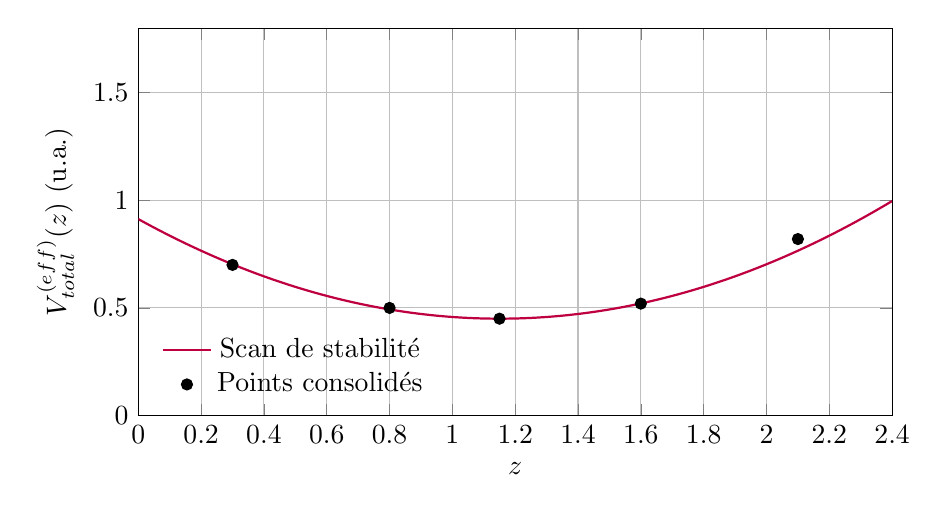
\begin{tikzpicture}
\begin{axis}[
    width=0.92\linewidth,
    height=6.5cm,
    xlabel={$z$},
    ylabel={$V_{total}^{(eff)}(z)$ (u.a.)},
    xmin=0, xmax=2.4,
    ymin=0.0, ymax=1.8,
    grid=both,
    legend style={at={(0.02,0.02)},anchor=south west,draw=none,fill=none},
]
\addplot[purple,thick,samples=120,domain=0:2.4] {0.35*(x-1.15)^2 + 0.45};
\addlegendentry{Scan de stabilité}
\addplot[only marks,mark=*,black] coordinates {(0.3,0.70) (0.8,0.50) (1.15,0.45) (1.6,0.52) (2.1,0.82)};
\addlegendentry{Points consolidés}
\end{axis}
\end{tikzpicture}